\documentclass{beamer}

\mode<presentation>
{
\usetheme{Boadilla}

\setbeamercovered{invisible}
}
\usecolortheme{crane}
\usepackage[utf8]{inputenc}
\usepackage[croatian]{babel}
\usepackage[T1]{fontenc}
\usepackage{booktabs}
\usepackage{mathptmx}
\usepackage[scaled=.90]{helvet}
\usepackage{courier}
\usepackage{multicol}


\usepackage[T1]{fontenc}


\title{Raspoznavanje preklapajućih 2D objekata}

\subtitle{Projekt iz Računalnog vida}

\author{Tomislav Babić \and Mateja Čuljak \and Đorđe Grbić \and Ivan Krišto \and Maja Šverko}

\institute[Universities of]
{
Fakultet Elektrotehnike i Računarstva\\
Sveučilište u Zagrebu}

\date{28.01.2011.}

% If you have a file called "university-logo-filename.xxx", where xxx
% is a graphic format that can be processed by latex or pdflatex,
% resp., then you can add a logo as follows:

% \pgfdeclareimage[height=0.5cm]{university-logo}{university-logo-filename}
% \logo{\pgfuseimage{university-logo}}

% Delete this, if you do not want the table of contents to pop up at
% the beginning of each subsection:
% \AtBeginSubsection[]
% {
% \begin{frame}<beamer>
% \frametitle{Outline}
% \tableofcontents[currentsection,currentsubsection]
% \end{frame}
% }

% If you wish to uncover everything in a step-wise fashion, uncomment
% the following command:

%\beamerdefaultoverlayspecification{<+->}

\begin{document}

\begin{frame}
\titlepage
\end{frame}

\begin{frame}
\frametitle{Pregled prezentacije}
\tableofcontents
% You might wish to add the option [pausesections]
\end{frame}


\section{Opis rješavanog problema}
\begin{frame}
\frametitle{Opis rješavanog problema}
\textbf{Problem:} Izgradnja sustava računalnog vida za klasifikaciju
preklapajućih 2D objekata.

Skup objekata koji se klasificiraju je unaprijed
poznat.

\pause
\vspace{10pt}
Pojam ``preklapanje'' podrazumjeva pravila:
\begin{itemize}
  \item objekti se međusobno preklapaju,
  \item moguće je da objekt ne sudjeluje u preklapanju (tj.\ objekt je samostalan),
  \item svaki objekt prekriven je najviše jednim objektom,
  \item razine preklapanja su proizvoljne,
  \item rotacija, skaliranje i pomak objekata su proizvoljni,
  \item boja objekta je proizvoljna.
\end{itemize}
\end{frame}

\section{Razvijeno rješenje}
\begin{frame}
\frametitle{Razvijeno rješenje}
Rješenje se temelji na radu \emph{HYPER: A new approach for the recognition and positioning of two-dimensional objects} (Ayache, N.\ i Faugeras, O.D.).

\pause
Skica postupka:
\begin{enumerate}
  \item<2-> \textbf{Inicijalizacija:} Segmentacija svakog modela (osnovni objekti).
  \item<3-> \textbf{Ulaz:} Segmentacija scene (slika sa preklapanjem).
  \item<4-> \textbf{Generiranje hipoteza:} kombiniranje svih segmenata svakog modela i scene.\\
  \textsc{Hipoteza:} uređena trojka afinih transformacija $\rightarrow$ $H=\left(k, (tx, ty), \beta \right)$
  \item<5-> \textbf{Evaluacija hipoteza:} računanje postotka preklapanja transformiranih modela i scene.\\
  Prilikom sparivanja segmenata hipoteza $H$ se ažurira metodom najmanjih kvadrata.
  \item<6-> \textbf{Izlaz:} Vjerojatnosti da se određeni model nalazi na sceni.
\end{enumerate}
\end{frame}

\subsection{Rješenja podproblema}
\begin{frame}
\frametitle{Razvijeno rješenje}
\framesubtitle{Rješenja podproblema (1)}
\textbf{Segmentacija:}
\begin{enumerate}
  \item binarizacija slike (jednostavne scene -- usporedba s fiksnim pragom),
  \item određivanje granica (\emph{Boundary Following Algorithm}),
  \item određivanje segmenata (\emph{Divide and conquer} algoritam, $\tau = 10$),
  \item stapanje segmenata koji leže na bliskim pravcima (prag: $\alpha = 15^\circ$).
\end{enumerate}
\pause
\textbf{Generiranje hipoteza:}
\begin{itemize}
  \item Za svaki model $m$:
  \begin{itemize}
    \item Svaki segment od $m$ upari sa svakim segmentom scene preko hipoteze $H$:
    \begin{align*}
      x^{\ast} & = tx + x\cdot k\cdot \cos(\beta) - y\cdot k\cdot \sin(\beta), \\
      y^{\ast} & = ty + y\cdot k\cdot \cos(\beta) + y\cdot k\cdot \sin(\beta).
    \end{align*}
    Točka modela $(x, y)$ se preslikava u točku scene $(x^{\ast}, y^{\ast})$ preko
    transformacija od $H$.
  \end{itemize}
  \pause
  (ako model ima 4 segmenta (npr.\ kvadrat), a scena 10 za taj model se generira 40 hipoteza!)
\end{itemize}
\end{frame}

\begin{frame}
\frametitle{Razvijeno rješenje}
\framesubtitle{Rješenja podproblema (2)}
\textbf{Evaluacija hipoteza:}
\begin{itemize}
  \item Za svaki par modela i hipoteze $(m, H)$:
  \begin{itemize}
    \item Iterativno se uspoređuju preostali linearni segmenti modela sa segmentima scene.
    \item Računa se različitost između segmenta modela i scene.\\
    Linearna kombinacija:
    \begin{itemize}
      \item razlike duljina,
      \item udaljenosti središnjih točki,
      \item relativne udaljenosti između duljina segmenata.
    \end{itemize}
    \item \textbf{Ažuriranje hipoteze:} tražimo transfomaciju $T$ koja minimizira kriterij
    $$R=\sum_i \frac{l_i}{K}\Delta^2(T(m_i),s_{ji}).$$
    Koristimo metodu najmanjih kvadrata.
  \end{itemize}
\end{itemize}
\pause
\textbf{Mjera kvalitete hipoteze:} Omjer duljine segmenata modela
sparenih s odgovarajućim segmentima u sceni i duljine svih segmenata modela.
\end{frame}

\section{Rezultati}
\begin{frame}
\frametitle{Rezultati}
\begin{itemize}
  \item Evaluacija je rađena nad 11 modela i sveukupno 105 slika.
  \item Svi objekti na sceni prepoznaju se u $40\%$ slučajeva.
  \item Barem jedan objekt na sceni prepozna se u $86.7\%$ slučajeva.
  \item Uspješnost referentne metode nije poznata!
\end{itemize}
\begin{table}[htb]
\centering
\caption{Uspješnost prepoznavanja po objektima.}
\label{tbl:po-obj}
\begin{tabular}{l l l l l l}
\toprule
 & 1 od 1 & 0 od 1 & 2 od 2 & 1 od 2 & 0 od 2\\
\midrule
Broj: & 21/22 & 1/28 & 21/83 & 49/83 & 7/83\\
Postotak: & $95.4\%$ & $3.6\%$ & $25.3\%$ & $59.0\%$ & $8.4\%$\\
\bottomrule
\end{tabular}
\end{table}
\end{frame}

\subsection{Analiza rezultata}
\begin{frame}
%\frametitle{Rezultati}
%\framesubtitle{Analiza rezultata (1)}
\begin{figure}[htb]
\begin{center}
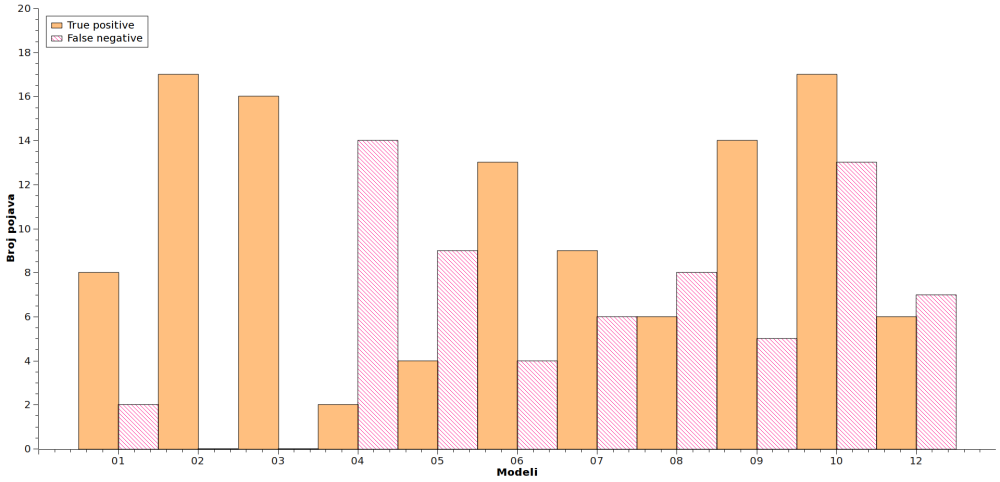
\includegraphics[width=9cm]{resources/graf.png}
\end{center}
\caption{Graf uspješnih i neuspješnih prepoznavanja po modelima.} 
\label{fig:graf}
\end{figure}

\begin{figure}[htb]
\begin{center}
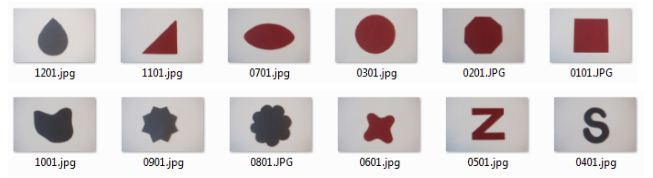
\includegraphics[width=8cm]{resources/baza.png}
\end{center}
\caption{Prikaz objekata za klasifikaciju.} 
\label{fig:baza}
\end{figure}
\end{frame}

\begin{frame}
%\frametitle{Rezultati}
%\framesubtitle{Analiza rezultata (1)}
\begin{figure}[!h]
\begin{center}
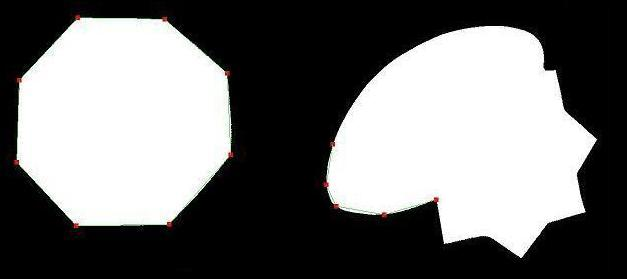
\includegraphics[width=7.5cm]{resources/oktagon-spoj.png}
\end{center}
\caption{Spajanje segmenata (kvaliteta $50.3\%$).} 
\label{fig:segmenti-treca}
\end{figure}
\begin{figure}[!h]
\begin{center}
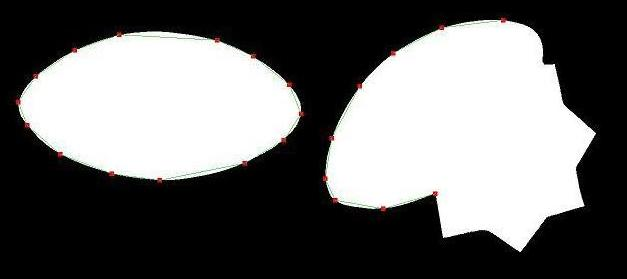
\includegraphics[width=7.5cm]{resources/elipsa-spoj.png}
\end{center}
\caption{Utjecaj skaliranja i rotacije (kvaliteta $49.5\%$).} 
\label{fig:segmenti-rotacija}
\end{figure}
\end{frame}

\section{Izdvojeni problemi}
\begin{frame}
\frametitle{Izdvojeni problemi}
\begin{itemize}
  \item \emph{Divide and conquer} algoritam nije invarijantan na rotaciju.
  \item Bilo je potrebno stopiti dio segmenata nakon prolaska \emph{divide and conquer} algoritma.
  \item Postupak je dosta osjetljiv na šum pri određivanju segmenata. 
  \item Postupak ne daje odgovor na pitanje ``\emph{Koliko je objekata na sceni?}.''
  \item Likovi u bazi su nakon određivanja segmenata postali previše slični (primjerice, oktagon i krug).
\end{itemize}
\end{frame}

\section{Moguća poboljšanja}
\begin{frame}
\frametitle{Moguća poboljšanja, nastavak rada}
\begin{itemize}
  \item Evaluiranje drugih metoda aproksimiranja konture (segmentiranja).
  \item Korištenje drugih transformacija pri generiranju hipoteza.
  \item Uvođenje dodatnih mjera za određivanje kvalitete hipoteza.
  \item Izgradnja heurističkih pravila za određivanje broja objekata koji se pojavljuju na slici.
  \item Proširenje metode za raspoznavanje preklapanja više od 2 objekta.
\end{itemize}
\end{frame}


\end{document}
